\chapter{Building a UPPAAL Model}
\section{Program Representation}
When translating a program to a UPPAAL of the program. Several representations are possible, depending on what one wants to show. One could for example represent a program merely in terms of program flow if a simulation of a disruption of the program flow is to be shown, e.g an error in the program counter. One could also include the data flow in the program if a simulation of a corruption of a memory value is to be shown. These are just a few examples and many representations can be chosen.\\

We have chosen the later and model the program in terms of program flow and data flow, so that we can simulation disruptions in the programs execution flow. 


\subsection{Representation Details}
The program simulation is based on \jcl semantics, most Java bytecodes can be translated directly to \jcl at the loss of type information.\\

When representing Java bytecode in UPPAAL we have chosen to represent an instruction, such as \texttt{aload a} and \texttt{dub}, as UPPAAL locations. 
This implies that a change in the program counter is a change of the location. 
In turn this means that when an instruction is to be executed the change to the program configuration \textit{Conf} from  \cref{sec:semintro} occurs on the edge to next location.

\begin{lstlisting}[caption=Jave code.]
public class Sample{
    public static void main(String[] args) {
        for (String a : args)         
        {
            System.out.print(a);
        }
    }
}
\end{lstlisting}

\begin{lstlisting}[caption=Bytecode.]
public static void main(java.lang.String[]);
 Code:
   0: aload_0       
   1: astore_1      
   2: aload_1       
   3: arraylength   
   4: istore_2      
   5: iconst_0      
   6: istore_3      
   7: iload_3       
   8: iload_2       
   9: if_icmpge     31
  12: aload_1       
  13: iload_3       
  14: aaload        
  15: astore        4
  17: getstatic     #2                  // Field java/lang/System.out:Ljava/io/PrintStream;
  20: aload         4
  22: invokevirtual #3                  // Method java/io/PrintStream.print:(Ljava/lang/String;)V
  25: iinc          3, 1
  28: goto          7
  31: return        

\end{lstlisting}

\subsubsection{Simple Instructions}
\begin{figure}[H]
\centering
\begin{subfigure}{.3\textwidth}
  \begin{lstlisting}
  0. aload 0
  1. arraylength
  ...
  \end{lstlisting}
  \caption{Java Bytecode Sample.}
\end{subfigure} 
\hspace{10px}
\begin{subfigure}{.6\textwidth}
  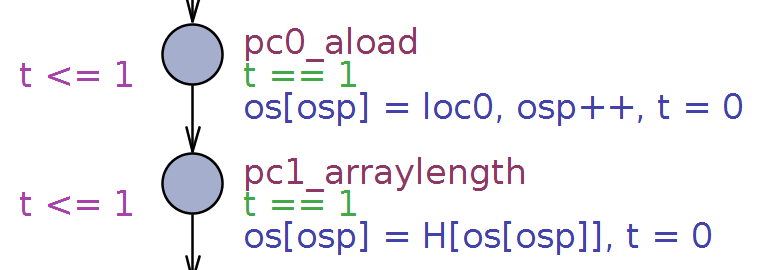
\includegraphics[width=\textwidth]{UPPAAL1.png}
  \caption{Generated model from Sample.}
\end{subfigure}
\caption{Java Bytecode and Corresponding UPPAAL Model.}
\label{fig:uppaal1}
\end{figure}
\kri{lav ny model til nyt smaple}
\Cref{fig:uppaal1} show how two Java Bytecode instructions are represented in UPPAAL. On the Left we see the Java bytecode, the first line with program counter 0 we have the \texttt{aload 0} instruction. \texttt{aload 0} pushes a reference to the top of the operation stack from local variables a position zero, then increments the operation stack pointer and program counter.

arraylength

uppaal location edge

update

invariant guard

\subsubsection{Jumps and Branches}
goto

conditionals
\subsubsection{Method Calls}
Method calls are represented by three additions to the model. These additions consist of locations, but they do not have any associated program counter since they are not a part of the original program.\\

% special case for main
The first is an addition of a location in the template of the \texttt{main} method. This location captures the notion that this is the start of the program.\\

% caller
The second is a new location in the caller for every method call it performs. This makes it possible to simulate parameter passing, as well as control transfer when waiting for a callee to return control to the caller after a method call. The simulation of the caller remains in this location until the callee returns control, after its simulation has finished. This control transfer is modeled with a synchronisation on the edge going from the new state in the caller and back to its original control flow.\ch{insert ref to figure}~\\

% callee
The third is an addition of a two initial locations in every template except for the \texttt{main} template. The first, initial, location serves dual purposes: it enables the control transfer from the caller to itself by synchronisation, and simulates passing of arguments into the method from the caller. The second location is the \textit{done} location, where the simulation ends up when it has finished its simulation. This is where control is transferred back to the caller.

\section{Modelling a Fault Injection}
\ch{mention in modelling a fault injection that there should not be any fault transitions going back to the added state since it does not have a program counter}